\section{Background} \label{sec:background}

\subsection{Deep End-to-End Control}
End-to-end training of deep neural network models is an active
research area in the fields of AI~\cite{Levine2016}.

\begin{figure}[h]
  \centering
  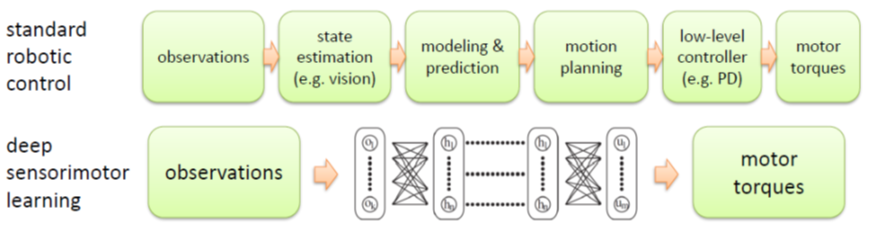
\includegraphics[width=.5\textwidth]{figs/endtoend}
  \caption{Standard robotics control vs. DNN based end-to-end
    control. \fixme{figure must be redrawn}}
\end{figure}

- explosion of AI
- in particular, application of DNN in perception and control of robotics systems.
- end-to-end control is a promising technique.
  levine's publications?
- examples: nvidia's DAVE-II prototype, forest navigating drone
challenge problem: computing at low cost?

%% UPenn's f1/10 BOM: $3,628.37	
%% http://f1tenth.org/
%% http://selfdrivingcars.mit.edu/
%% http://fast.scripts.mit.edu/racecar/
%% https://github.com/mit-racecar
%% https://mit-racecar.github.io/

\subsection{Embedded Multicore Single-Board-Computers}

- computing has been a obstacle.
- performance, but also constraints size, weight, and power as well as
cost senstive nature of industries including automtive.
- many new embeded computing platforms emerged: affordable and
powerful. raspberry pi, nvidia's embedded platforms tout their
superiority in GPU based acceleration of the AI tasks.

Our primary objective of this study are
- to understand the necessary computing performance for applying AI
technology based robotics systems, and 
- what kind of computing architecture and runtime supports
are most appropriate for such workload.

Toward to achieve the two goals, we implement a low-cost autonomous
car platform as a case study, as we will explain in the following
section. 
